\documentclass[a4paper,fleqn]{cas-dc}

\usepackage[authoryear,longnamesfirst]{natbib}
\usepackage{amsmath,amssymb}
\usepackage{xcolor}
\usepackage{placeins}
\usepackage{xurl}   % lets long URLs break across lines
\graphicspath{{./}{../}}   % figures live in ../figs when compiling from report/

% ---------------------------------------------------------------------------
% Markers for results that are still being run. Search for \pending and
% \provisional before submission; delete the two lines below to hide them.
\newcommand{\pending}[1]{\textcolor{red}{[PENDING: #1]}}
\newcommand{\provisional}[1]{\textcolor{red}{#1}}
% ---------------------------------------------------------------------------

\ExplSyntaxOn
\cs_set:Npn \__first_footerline:
  { \group_begin: \small \sffamily \__short_authors: :~ { \rmfamily \itshape Honours~Research~Report } \group_end: }
\ExplSyntaxOff
\RenewDocumentCommand\printorcid{}{}

\newcommand{\KL}{D_{\mathrm{KL}}}
\newcommand{\Pa}{\mathrm{Pa}}

\begin{document}
\let\WriteBookmarks\relax

\renewcommand{\textfraction}{.3}
\renewcommand{\topfraction}{.70}
\renewcommand{\bottomfraction}{.50}
\renewcommand{\floatpagefraction}{.60}
\renewcommand{\dbltopfraction}{.60}
\renewcommand{\dblfloatpagefraction}{.60}

\shorttitle{Neural Parameter Estimation for Discrete Bayesian Networks}
\shortauthors{K. Aspoas}

\title [mode = title]{Neural Network Parameter Estimation for Discrete Bayesian Networks with Applications in Medical Diagnosis}



\author[1]{Kaylin Aspoas}
\author[1]{Ritesh Ajoodha\texorpdfstring{\,\textnormal{\itshape (Supervisor)}}{ (Supervisor)}}
\author[1]{Aashna Gaogle\texorpdfstring{\,\textnormal{\itshape (Co-supervisor)}}{ (Co-supervisor)}}

\affiliation[1]{organization={School of Computer Science and Applied Mathematics, University of the Witwatersrand},
            city={Johannesburg},
            country={South Africa}}


\begin{abstract}
Bayesian networks offer an interpretable framework well-suited to medical diagnosis, but their standard parameter estimation methods estimate a separate distribution for every configuration of a variable's parents, and become unreliable when data is scarce relative to the number of configurations. This research replaces the conditional probability table (CPT) at each node with a neural conditional probability distribution (neural CPD), a small neural network that shares parameters across parent configurations while preserving the interpretable graph structure. On synthetic networks whose CPTs share no structure across configurations, a smoothed CPT matched to the generating prior is optimal by construction; neural CPDs, which are not told that prior, stay within about two and a half times its divergence and beat unsmoothed maximum likelihood in nearly every setting. When the synthetic CPTs do share structure, neural CPDs beat even a validation-tuned smoothed CPT once nodes have six or more parents, with up to 4.4 times lower divergence. On a real clinical dataset with expert-elicited structures, neural CPDs outperform a validation-tuned smoothed CPT in held-out log-likelihood in all 108 cross-validated settings, and the smoothed CPT needs 3 to 67 times as much data to match them. They also predict diabetes far more accurately, because the diabetes node has the largest CPT in every expert graph.
\end{abstract}

\begin{keywords}
Bayesian networks \sep Parameter estimation \sep Neural networks \sep Medical diagnosis
\end{keywords}

\maketitle

% ===========================================================================
\section{Introduction}\label{sec:intro}
% ===========================================================================

Predictive models are increasingly used to support medical decision making, which raises a difficult question: who is to blame when they get it wrong? In medicine, a diagnosis must be something that can be explained, questioned and justified. If a model contributes to a missed diagnosis and there is no reasoning to inspect, responsibility becomes difficult to assign, and a clinician has no way of knowing whether the model learned a medically meaningful relationship or an accidental pattern. Yet such models remain valuable, because diagnosis depends on many interacting factors, such as symptoms, test results, history and lifestyle, and a well-designed model can find patterns that would otherwise be missed. The aim is therefore to support clinical judgement in a way that remains understandable and accountable.

Bayesian networks offer a promising way to do this, because they represent medical reasoning as a visible structure of relationships that shows how each piece of information contributes to a diagnosis. However, traditional Bayesian networks struggle when these relationships become complex. Each variable's relationship to its causes is learned as a separate probability for every combination of those causes, and as the number of combinations grows, the data available to estimate each one shrinks. Deep learning models capture complex patterns but are hard to interpret, while Bayesian networks are easy to understand but limited by how they learn. This research investigates whether neural networks can be used inside the interpretable structure of a Bayesian network to combine these strengths.

The contribution of this work is threefold. First, it confirms under controlled conditions that the failure of tabular estimators such as Maximum Likelihood Estimation (MLE) is governed by the number of training rows per parent configuration, which falls as in-degree or cardinality increases, or as sample size decreases. Second, it evaluates neural conditional probability distributions (CPDs) as a drop-in replacement for conditional probability tables (CPTs) on synthetic networks. Without being told how the networks were generated, they stay within about two and a half times the divergence of the optimal smoothed CPT and comfortably beat unsmoothed MLE, and when parent configurations share structure they outperform even a validation-tuned smoothed CPT at high in-degree. Third, on a real clinical dataset with expert-elicited structures, they outperform a validation-tuned smoothed CPT in every setting tested, matching it with 3 to 67 times less data, and substantially improve the diagnosis of diabetes.

Section~\ref{sec:related} reviews related work, Section~\ref{sec:method} describes the methodology, Section~\ref{sec:results} presents the results, and Section~\ref{sec:conclusion} concludes and outlines future work.

% ===========================================================================
\section{Related Work}\label{sec:related}
% ===========================================================================

Approaches to estimating the conditional distributions of a Bayesian network differ mainly in how much they share between parent configurations. Tabular estimators share nothing, structured estimators share in ways fixed in advance, and neural networks learn what to share, a difference that matters most in clinical networks with many interacting risk factors.

\subsection{Tabular Parameter Estimation}

Parameter learning in Bayesian networks with a known DAG reduces to estimating node-wise conditional probability distributions independently. In discrete BNs, MLE estimates each CPT entry as a ratio of observed counts \citep[Sec.~17.2]{koller2009probabilistic},
\begin{equation}
\hat{P}(X_i = x_k \mid \Pa(X_i)=u_j)=\frac{N_{ijk}}{N_{ij}},
\label{eq:mle}
\end{equation}
where $N_{ijk}$ counts the samples in which $X_i=x_k$ and $\Pa(X_i)=u_j$. This works well when data is abundant, but zero-valued parameters from unobserved configurations propagate through inference and suppress otherwise valid conclusions \citep{impact_oniko_2013}. Because a variable with $k$ parents of cardinality $r$ has $r^k$ configurations, even moderate in-degree produces tables too large to estimate from finite data \citep[Sec.~5.2]{learning_oniko_2001,koller2009probabilistic}.

Bayesian parameter estimation (BPE) with Dirichlet priors ensures non-zero probabilities \citep[Secs.~17.3--17.4]{koller2009probabilistic}. The strength of the prior, such as the equivalent sample size of the BDeu prior \citep{heckerman1995learning}, must still be chosen, and informative priors are impractical to specify at the scale of clinical networks \citep{comprehensive_kyrimi_2021}. Constraint-based priors such as CaMAP improve on uniform Dirichlet priors but require expert-provided parameter constraints \citep{constrained_di_2021}. Whatever the prior, each parent configuration is still estimated from its own counts, so a configuration that is rarely or never observed is left close to the prior.

\subsection{Structured Parameter Estimation}

Structured estimators reduce the number of free parameters by letting parent configurations share them. Noisy-OR gates make the number of parameters linear in the number of parents for binary variables, at the cost of independence assumptions that rarely hold exactly \citep{learning_oniko_2001}. Local structure, such as decision trees or default tables inside a CPT, ties together configurations that behave alike and gives more robust estimates from small samples \citep{friedman1996learning}. Hierarchical Dirichlet processes smooth each configuration's estimate towards those of configurations that share some of its parent values, which makes Bayesian network classifiers competitive with random forests \citep{petitjean2018accurate}.

\subsection{Neural Networks in Probabilistic Models}

Each of these methods imposes a particular form of sharing: an independence assumption, a tree over parent values, or a hierarchy over them. Parametric models instead learn the conditional distribution as a function of the parents, and the simplest neural CPD has no hidden layer. Sigmoid belief networks make each binary node a logistic function of its parents \citep{neal1992connectionist}, and \citet{rijmen2008bayesian} replaced each CPT of a discrete network with a multinomial logistic regression on its parents; logistic and other generalised linear CPDs are now standard textbook models \citep[Ch.~5]{koller2009probabilistic}. A multinomial logistic CPD is the linear softmax used as a control in this report: it shares parameters across all configurations, but its log-probabilities are additive in the parents unless interaction terms are specified by hand, which grows the model back towards the full table.

A hidden layer removes the need to specify interactions in advance. \citet{bengio2000taking} and the neural autoregressive distribution estimator \citep{larochelle2011neural} model high-dimensional discrete data as a product of conditionals computed by networks with a hidden layer, but they condition each variable on all earlier variables in an ordering rather than estimating the CPDs of a given graph. Per-variable networks on a DAG appear in causal discovery: \citet{ke2019learning} model each categorical variable with a one-hidden-layer network whose one-hot inputs are masked by a hypothesised graph and whose softmax output gives the conditional distribution, but they use it to learn the graph from interventions rather than to estimate parameters on a fixed one. Closest to this report, \citet{Gaogle2026} replaced the linear-Gaussian CPDs of Gaussian BNs with neural networks and found them competitive with classical baselines, including ridge regression, but the Gaussian setting assumes continuous, jointly normal variables, whereas clinical variables such as symptom presence and categorical risk levels are discrete.

\subsection{Bayesian Networks in Medical Diagnosis}

The estimation problem is especially pressing in medicine, where BNs are widely applied to diagnosis and risk prediction because their graphical structure makes probabilistic reasoning visible and inspectable \citep{comprehensive_kyrimi_2021,zhong2024predicting}. Interpretability is a requirement for safe clinical decision making \citep{explainable_hulsen_2023}, and post-hoc explanations of black-box models are criticised as unfaithful to the model's reasoning \citep{stop_rudin_2019}. The structure of a clinical network is often elicited from experts rather than learned: \citet{zahoor2025investigatingvaliditystructurelearning} elicited diabetes DAGs from domain experts at three levels of confidence, which this report uses as fixed structures. Clinical variables are also often collapsed into a few coarse categories, as in the published discretisation of these diabetes data \citep{zahoor2025investigatingvaliditystructurelearning}, which keeps the CPTs small enough to estimate but discards information the experts' graph could otherwise use.

No previous work evaluates neural CPDs as a replacement for the CPTs of a fixed, expert-given discrete network, against smoothed tabular estimators whose prior is chosen on validation data. This report does so. Its neural CPD maps the one-hot-encoded parents through a hidden layer to a softmax output, sharing parameters across parent configurations while preserving the DAG factorisation, and the linear softmax isolates what the hidden layer adds.

% ===========================================================================
\section{Methodology}\label{sec:method}
% ===========================================================================

The estimators are compared on synthetic networks, where the true parameters are known, and on a clinical dataset, where they are not. Both settings share the same estimation problem.

\subsection{Problem Formulation}

A Bayesian network is defined by a directed acyclic graph $G$, where each node has an associated conditional probability distribution, and the joint distribution factorises according to $G$ as
\begin{equation*}
P(X_1,\dots,X_n)=\prod_{i=1}^{n} P(X_i\mid\Pa_{X_i}),
\end{equation*}
where $\Pa_{X_i}$ denotes the parents of $X_i$ in $G$ \citep{koller2007graphical}.

The factorisation lets each CPD be estimated separately, from the columns of its node and that node's parents. Tabular estimators such as MLE and BPE go further and estimate a separate distribution for every parent configuration. A variable with $k$ parents of cardinality $r$ has $r^k$ parent configurations, so with $N$ training rows each configuration is observed on average $\rho$ times, where
\begin{equation}
\rho = \frac{N}{r^{k}}.
\label{eq:rho}
\end{equation}
Increasing in-degree or cardinality, or reducing the sample size, all reduce $\rho$ in the same way. Once $\rho$ falls near or below one, most configurations are seen rarely or never, and tabular estimates fall back on their defaults. Clinical networks often reach this regime, because diagnoses depend on many interacting factors while clinical data does not grow to match. The aim is a parameter estimator that remains reliable when $\rho$ is small while keeping the graph, and so the interpretability, of the BN.

The evaluation has two parts. On synthetic networks with known parameters, estimators are compared under controlled in-degree, cardinality and sample size. On a real clinical dataset with expert-elicited structures, the same estimators are compared under three discretisations, which vary $\rho$ through cardinality with the graph held fixed.

\subsection{Estimators}\label{sec:estimators}\label{sec:archsel}

MLE estimates each CPT with Eq.~\eqref{eq:mle}. A parent configuration that never appears in the data is assigned a uniform distribution, and a child state never observed under an observed configuration keeps a probability of zero.

BPE avoids these zeros by adding a symmetric Dirichlet pseudocount $a$ to every cell before normalising, $\hat P = (N_{ijk}+a)/(N_{ij}+ar)$. The Dirichlet estimator uses $a=0.5$, the same value as the $\alpha$ that generates the synthetic CPTs (Section~\ref{sec:synthetic}). Because every synthetic CPT column is an independent $\mathrm{Dir}(0.5,\dots,0.5)$ draw, this estimator is the exact posterior mean of each column and minimises expected KL divergence from the ground truth. On synthetic data it is therefore a \emph{matched-prior reference}, the best achievable by any estimator given the data, rather than a competitor that neural CPDs are expected to beat. The Laplace estimator uses $a=1$, a standard default that does not depend on the generator, and shows how much of the reference's advantage comes from knowing $\alpha$. Where no fixed pseudocount is optimal, on the structured ground truths and on real data, the pseudocount is chosen on validation data.

A neural CPD replaces the CPT of each node $X_i$ with a network $f_\theta$ that maps the parents to a distribution over the states of $X_i$ (Figure~\ref{fig:neuralcpd}),
\begin{equation*}
P(X_i\mid\Pa(X_i))=f_\theta(\Pa(X_i)).
\end{equation*}
Each parent is one-hot encoded at its own cardinality and the encodings are concatenated, so the input width grows with the \emph{sum} of parent cardinalities rather than their product. A root node receives a constant input and learns its marginal through the output bias. Hidden layers use ReLU activations, and a softmax output gives a valid distribution. Because the log-likelihood of a Bayesian network is a sum of one term per node, one network is trained per node by minimising the cross-entropy
\begin{equation*}
\mathcal{L}(\theta)=-\frac{1}{N}\sum_{s=1}^{N}\log P_\theta\big(x_i^{(s)} \mid \mathrm{pa}_i^{(s)}\big),
\end{equation*}
where $x_i^{(s)}$ and $\mathrm{pa}_i^{(s)}$ are the observed state and parent configuration in row $s$.

\begin{figure}[pos=tbp]
\centering
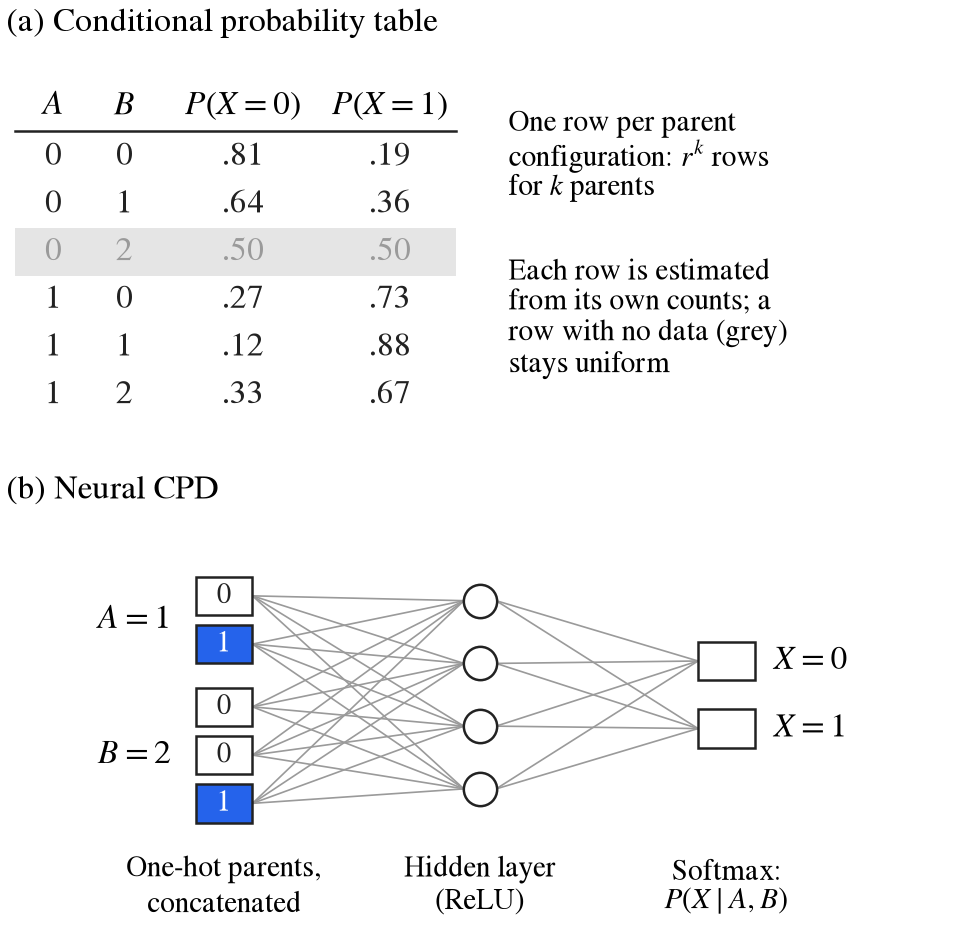
\includegraphics[width=\columnwidth]{figs/neural_cpd.png}
\caption{One node $X$ with parents $A$ (two states) and $B$ (three states). (a) Its CPT has one row per parent configuration, each estimated from that configuration's rows alone. (b) The neural CPD encodes each parent as a one-hot vector, concatenates them, and maps them through a ReLU hidden layer to a softmax over the states of $X$, so every configuration shares the same weights.}\label{fig:neuralcpd}
\end{figure}

All networks are trained on mini-batches with AdamW \citep{loshchilov2019decoupled}, except the linear softmax, which uses Adam \citep{kingma2015adam} at its default settings. A share of the $N$ rows is held out for early stopping (30\% on synthetic data, 20\% on real data), and each node stops independently on its validation loss. The tabular estimators fit on all $N$ rows, so the networks see fewer rows, not more.

Table~\ref{tab:estimators} lists the estimators. The linear softmax has no hidden layer, so it is a multinomial logistic regression fitted per node: it shares parameters across configurations but cannot represent interactions between parents, and acts as a control for the effect of the hidden layer. It is run at untuned default settings.

The other networks were configured separately for each cardinality on tuning DAGs that are disjoint from the evaluation DAGs, using only validation loss. An initial run without early stopping showed that larger networks overfit quickly, so every network uses early stopping. Bayesian hyperparameter sweeps at in-degrees 2, 6 and 10 then selected six architectures at $r=2$ and five at $r=4$, with one or two hidden layers of 32 to 256 units; in both sweeps the best configurations had 256 units or two hidden layers. The tuning results and every network's settings are given in the supplementary material (Supplementary Figures~S1--S2 and Tables~S1--S2). The main comparison uses \texttt{nn\_32}, a single hidden layer of 32 units and the smallest of the tuned networks.

\begin{table}[tbp]
\caption{Estimators. All networks use ReLU hidden layers and per-node early stopping; settings for each network and cardinality are in Supplementary Table~S2.}\label{tab:estimators}
\begin{tabular*}{\tblwidth}{@{\extracolsep{\fill}}ll@{}}
\toprule
Estimator & Description \\
\midrule
MLE & CPT; uniform for unseen configurations \\
Dirichlet & CPT, pseudocount 0.5 \\
Laplace & CPT, pseudocount 1 \\
Dirichlet (tuned) & CPT, pseudocount chosen on validation data \\
\texttt{nn\_linear} & Linear softmax (no hidden layer), untuned \\
\texttt{nn\_32} & One hidden layer of 32 units \\
Tuned MLPs & One or two hidden layers of 32--256 units \\
\bottomrule
\end{tabular*}
\end{table}

\subsection{Synthetic Experiments}\label{sec:synthetic}

Synthetic networks have known parameters, so the learned distributions can be compared directly with the true ones, which is not possible on real data. The DAGs are generated to control in-degree directly. The $n$ nodes are placed in a random order, and the node at position $i$ is given $\min(k,i)$ parents, chosen uniformly from the nodes before it, so every node past the first $k$ has in-degree exactly $k$.

Every column of every ground-truth CPT is drawn independently from a symmetric Dirichlet distribution, $P^*(X_i\mid \mathrm{pa}) \sim \mathrm{Dir}(\alpha,\dots,\alpha)$, with $\alpha=0.5$. Because the columns are independent, the rows observed under one parent configuration carry no information about any other. Sharing parameters across configurations therefore cannot help in expectation, and the best an estimator can do is the matched-prior reference. These networks test how close an estimator comes to that optimum without being told the prior.

To test whether neural CPDs gain when configurations do share structure, a second family of ground truths uses the same 20-node DAGs at $r=2$, with the same sample sizes and seeds. Each CPT is logistic: the score of each child state is the sum of a bias, one effect per parent and, optionally, effects for a few random pairs of parents, and the CPT column is the softmax of the scores. Configurations that agree on a parent therefore share that parent's effect. Two levels are used: purely additive CPDs, and CPDs in which half of the score variance comes from pairwise interactions. The score scale is set so that the columns are, on average, as sharp as Dirichlet(0.5) draws.

Table~\ref{tab:grid} lists the settings, which are crossed in full for every estimator, giving 500 configurations at $r=2$ and 300 at $r=4$. The number of training rows is held fixed as in-degree increases, so that any change in performance reflects the size of the conditional probability space rather than the amount of data. Training sets are drawn by ancestral sampling and nested, so the smaller sets are the first $N$ rows of the largest. A separate test sample of 10\,000 rows from each ground truth is used only to estimate KL divergence. Every random step has its own seed derived from the configuration, so all estimators see the same networks and data.

\begin{table}[tbp]
\caption{Synthetic experimental grid. Every setting is crossed in full for every estimator: 500 configurations at $r{=}2$ and 300 at $r{=}4$, which uses the values marked $\dagger$.}\label{tab:grid}
\begin{tabular*}{\tblwidth}{@{\extracolsep{\fill}}ll@{}}
\toprule
Setting & Values \\
\midrule
Network size $n$ & 10$^\dagger$, 20$^\dagger$, 30$^\dagger$, 40, 50 \\
Parent in-degree $k$ & 2$^\dagger$, 4$^\dagger$, 6$^\dagger$, 8$^\dagger$, 10$^\dagger$ \\
Dirichlet $\alpha$ & 0.5$^\dagger$ \\
Training rows $N$ & 200$^\dagger$, 600$^\dagger$, 1000$^\dagger$, 1400$^\dagger$ \\
Cardinality $r$ & 2, 4$^\dagger$ \\
DAGs per setting & 5 \\
Test sample (KL only) & 10\,000 rows \\
\bottomrule
\end{tabular*}
\end{table}

\subsection{Real Clinical Data}\label{sec:realdata}

The real-data experiments use the CDC Diabetes Health Indicators dataset \citep{cdc_diabetes_2023}, drawn from the 2015 Behavioral Risk Factor Surveillance System (BRFSS): 253\,680 survey responses across 21 health-related variables and a binary diabetes indicator. The structures are the expert-elicited diabetes DAGs of \citet{zahoor2025investigatingvaliditystructurelearning} at three levels of expert confidence (Supplementary Figure~S3). The high-confidence graph has 37 edges and a maximum in-degree of 7, the moderate-confidence graph has 50 edges and a maximum in-degree of 8, and the low-confidence graph has 55 edges and a maximum in-degree of 12. Only the DAG comes from the experts; all parameters are learned.

Every variable except body mass index is natively categorical, so the discretisations follow the survey instrument. The coarsest level (L1) reproduces the collapsed categories of \citet{zahoor2025investigatingvaliditystructurelearning} and matches their published marginals to within one percentage point. L2 uses the categories as collected, for example 13 age bands and 8 income bands, and L3 bins body mass index into deciles and the day-count variables more finely. The decile cut points are computed from each training fold alone, and are the same in every fold. Across the nine combinations of discretisation and DAG, the CPTs hold from 1\,348 free parameters (L1, high confidence) to over 9 million (L3, low confidence).

Estimators are compared by three-fold cross-validation, stratified on diabetes status. Within each training fold, nested subsets of $N\in\{500, 2000, 10\,000, 50\,000\}$ rows are drawn, and the whole held-out fold is the test set. The networks are \texttt{nn\_32} and \texttt{nn\_128\_64} with their $r=4$ settings, together with the untuned linear softmax. Because the real-data subsets are far larger than the tuning sets, the batch size grows in proportion to $N$ by a rule fixed before any run, so that the number of optimisation steps per epoch stays close to that at tuning.

Two hyperparameters are tuned by nested cross-validation: each network's learning rate ($3\times10^{-4}$, $10^{-3}$ or $3\times10^{-3}$) and the Dirichlet pseudocount (0.1, 0.5 or 1.0). Within each outer fold, each candidate is scored by its log-likelihood on the validation 20\% of each subset, averaged over all 36 combinations of discretisation, DAG and $N$, and the best is selected separately in each fold. A single value per fold is used because one combination's validation set can be as small as 100 rows, and because a pseudocount encodes a prior belief that should not depend on $N$. The selected candidate is refitted with the same rows and scored once on that fold's test set, which plays no part in any choice. Every fold selected a learning rate of $3\times10^{-3}$ for both networks and a pseudocount of 1.0, in each case the largest value in its grid.

\subsection{Evaluation}\label{sec:eval}

On synthetic data, the metric is the Kullback-Leibler divergence from the ground-truth joint distribution $P^*$ to the learned distribution $\hat P$ \citep[App.~A.1.3]{koller2009probabilistic}. The sum over all $r^n$ joint states is intractable, so the chain-rule decomposition is used, with a Monte Carlo estimate over the $S=10\,000$ test rows $x^{(s)}\sim P^*$:
\begin{align*}
\KL(P^*\|\hat P) &= \mathbb{E}_{P^*}\Big[\sum_{i} \KL\big(P^*_{i}\,\|\,\hat P_{i}\big)\Big] \\
&\approx \frac{1}{S}\sum_{s=1}^{S}\sum_{i=1}^{n}\sum_{x_i} P^*_{is}(x_i)\log\frac{P^*_{is}(x_i)}{\hat P_{is}(x_i)},
\end{align*}
where $P^*_{is}(x_i) = P^*(x_i\mid \mathrm{pa}_i^{(s)})$ is the true distribution of $X_i$ given its parents in row $s$, and $\hat P_{is}$ is the learned one. Only the parent configurations are sampled; the sum over each child's states is exact. Because KL is summed over nodes it grows with network size, so results that pool settings use a single network size (30 nodes).

Where MLE assigns zero probability to a child state with positive true probability, the divergence is infinite, so such zeros are floored at $\epsilon=10^{-12}$, as in other evaluations of unsmoothed estimators \citep{nafar2025extracting}; the same floor applies to MLE on the real data. Most of MLE's divergence then comes from these floored cells, so its size depends on $\epsilon$, and $\epsilon=10^{-6}$ roughly halves it. MLE is therefore reported as a reference for the cost of not smoothing, and quantitative comparisons rest on the smoothed estimators, which never assign zero probability, as in \citet{niculescu2006bayesian}.

On real data the ground truth is unknown, so performance is measured by the mean held-out log-likelihood per row, $\frac{1}{S}\sum_s\sum_i \log\hat P(x_i^{(s)}\mid\mathrm{pa}_i^{(s)})$. Its expected negative is the cross-entropy $H(P^*,\hat P) = H(P^*) + \KL(P^*\,\|\,\hat P)$, and $H(P^*)$ does not depend on the estimator, so differences in log-likelihood are exactly differences in KL divergence. The unseen-configuration rate, the fraction of test rows in which at least one node's parent configuration never occurs in training, is also reported. For diagnosis, the probability of diabetes given every other variable is computed exactly from the Markov blanket of the diabetes node, its own CPD and that of its single child, and scored by the area under the ROC curve (AUROC) and the log-loss.

Free parameters are counted as $(r-1)$ times the number of configurations for a CPT, and every weight and bias for a network. Training time is recorded in separate serial runs, since parallel execution inflates wall-clock times: on synthetic data for one 20-node network at in-degrees 2, 6 and 10 with $N\in\{600,1400\}$, and on real data for three settings spanning the size of the CPTs.

\section{Results}\label{sec:results}

The synthetic networks come first, because their known parameters show directly how each estimator behaves. The clinical data then test whether the same behaviour holds where the ground truth is unknown, followed by the cost of each estimator and a summary of the findings.

\subsection{Synthetic Networks}

In all synthetic results except the last subsection, the true distribution of each parent configuration is drawn independently. The results begin with the problem that neural CPDs are meant to address: how tabular estimators degrade as parent configurations outnumber the training rows.

\subsubsection{How Tabular Methods Fail}

The synthetic setup reproduces the well-known behaviour of tabular estimators under sparse data \citep[Sec.~17.2]{learning_oniko_2001,koller2009probabilistic}. Figure~\ref{fig:mle} shows that KL divergence and CPT memory both rise sharply once a node's parent configurations ($2^k$) outnumber the training rows. In 40-node networks, MLE's KL divergence rises from 0.28 to 58 nats and its memory from 2.5 to 508\,KB as in-degree goes from 2 to 10. The Dirichlet estimator removes the zero probabilities and has about fifteen times lower error at $k=10$, but follows the same pattern, rising from 0.07 to 3.81 nats.

\begin{figure*}[pos=tbp]
\centering
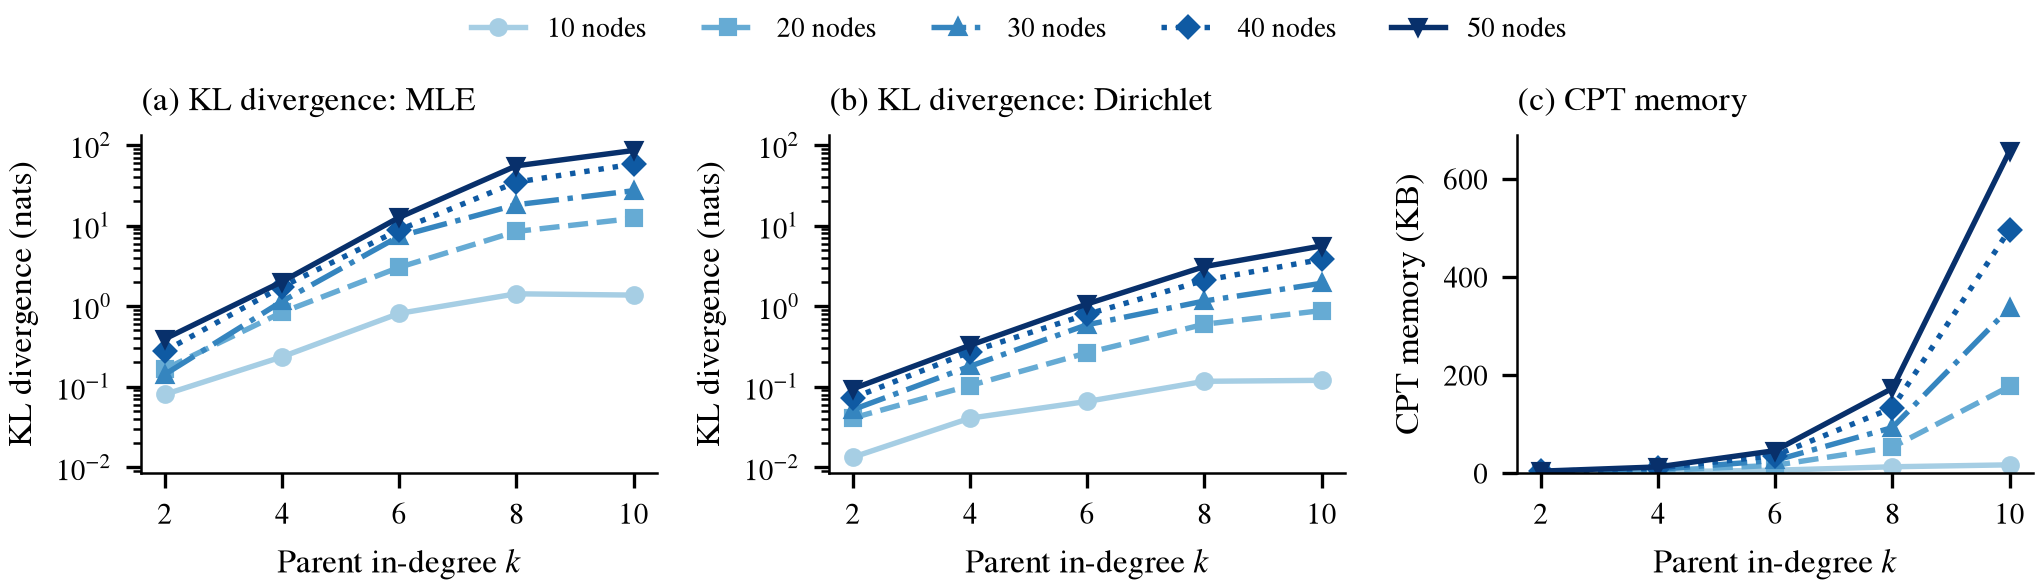
\includegraphics[width=\textwidth]{figs/mle_fails_c2.png}
\caption{Tabular estimators on synthetic networks ($r=2$) as in-degree increases ($N=1000$, $\alpha=0.5$, mean over five DAGs; darker is larger). KL divergence to the ground truth for (a) MLE and (b) the Dirichlet estimator (shared log-scaled y-axis). (c) Total CPT memory, the same for both.}\label{fig:mle}
\end{figure*}

The cause is data coverage rather than computation. In 20-node networks at $N=1000$, the share of parent configurations never seen in training rises from 0.5\% at $k=2$ to 78\% at $k=10$, while every MLE fit takes under one second. Both tabular estimators assign a uniform distribution to every unseen configuration, so smoothing removes zero probabilities but cannot recover these columns.

\subsubsection{Neural CPD Architectures}

Figure~\ref{fig:arms} compares every neural architecture with the tabular estimators at $r=2$. Every MLP has lower KL divergence than MLE at every in-degree, and the gap widens as the configuration space grows, while all of them stay above the matched-prior Dirichlet reference. The $r=4$ grid shows the same ordering. The MLPs differ little from one another, and no single architecture is best everywhere: at $r=2$, \texttt{nn\_256} is the best tuned network in 237 of the 500 configurations and \texttt{nn\_128\_64} in 97.

\begin{figure*}[pos=tbp]
\centering
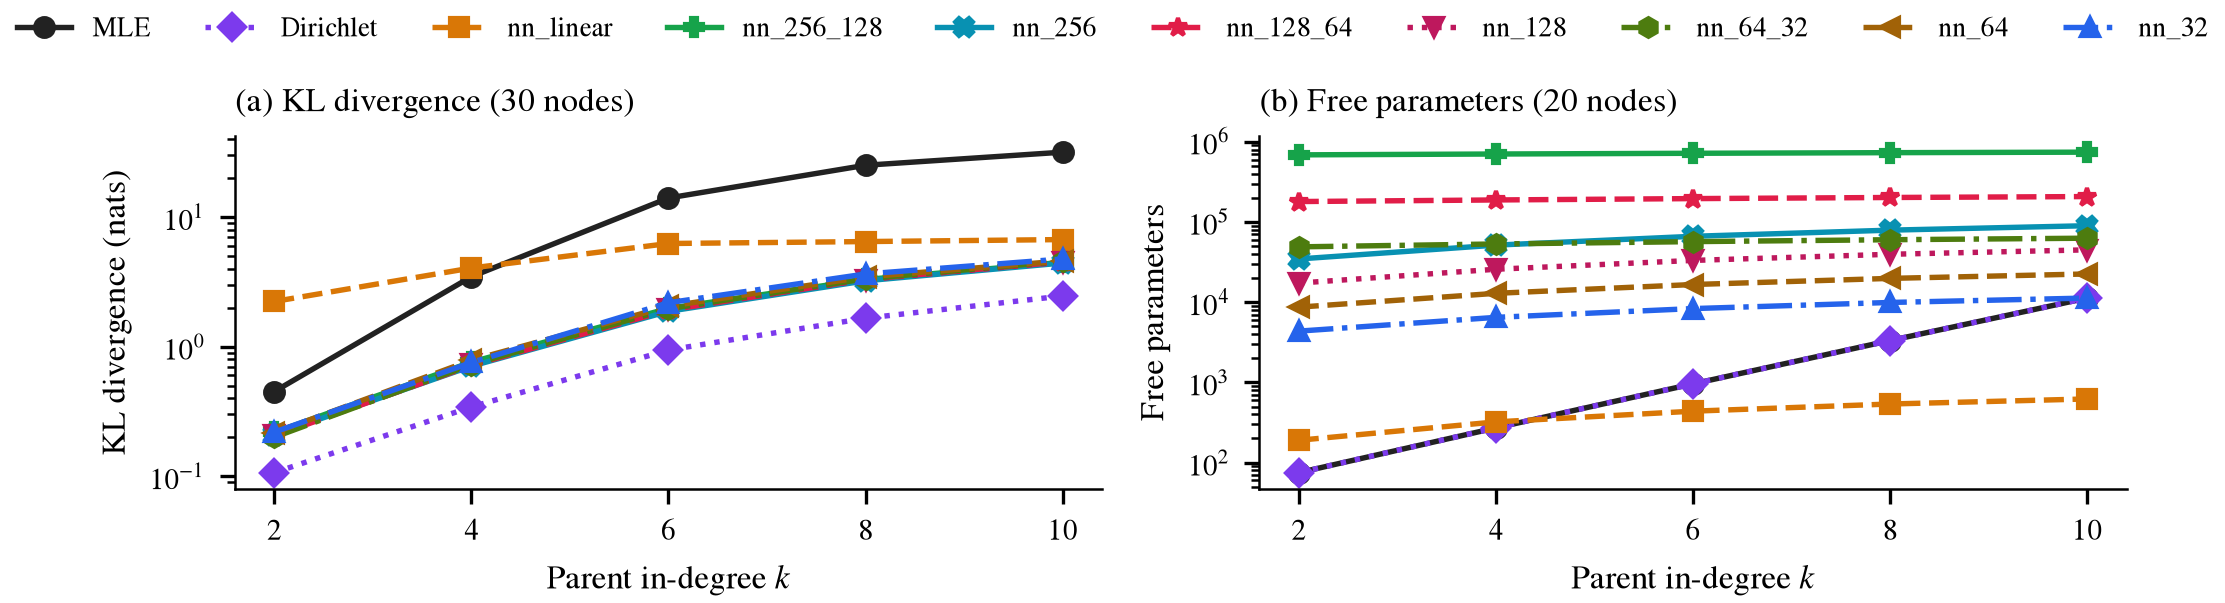
\includegraphics[width=\textwidth]{figs/arms_c2.png}
\caption{All estimators at $r=2$ ($\alpha=0.5$, mean over sample sizes and five DAGs; log-scaled y-axes). (a) Mean KL divergence against parent in-degree $k$ for 30-node networks; standard errors across the five DAGs are 1--12\% of each mean, smaller than the markers. (b) Free parameters for a 20-node network.}\label{fig:arms}
\end{figure*}

The linear softmax behaves differently. At $r=2$ it beats MLE in only 8\% of configurations at $k=2$, and overtakes it only once the configuration space is large (72\% at $k=6$ and 98\% at $k=8$). Its error also barely falls as more data is added (Figure~\ref{fig:klN}), which is the signature of bias rather than variance. Because the ground-truth CPT columns are drawn independently, the true conditionals contain full interactions between parents, which an additive model cannot fit. Sharing parameters therefore helps only when the shared model is flexible enough to represent the true conditionals, and the hidden layer provides that flexibility.

Because the MLPs differ little in accuracy but greatly in size (Figure~\ref{fig:arms}b), the smallest, \texttt{nn\_32}, is used for the remaining comparisons. Its KL divergence is on average 17\% above that of the best tuned network at $r=2$ and 8\% above at $r=4$, while it holds 2 to 66 times fewer parameters than the tuned architectures at $k=10$.

\subsubsection{Comparison with Tabular Estimators}\label{sec:compare}

Figure~\ref{fig:klN} shows how each estimator responds to more data. More rows help MLE, but at high in-degree it stays far worse than \texttt{nn\_32}, while at $k=2$ the two improve at a similar rate. Across the $r=2$ grid, \texttt{nn\_32} beats MLE in 493 of 500 configurations (98.6\%), rising from 93\% at $k=2$ to 100\% at $k\geq4$, and at $r=4$ it beats MLE in all 300. The ordering of the estimators is the same at every network size; larger networks change only the scale of the KL divergence, which is summed over nodes (Supplementary Figures~S4 and~S5).

\begin{figure*}[pos=tbp]
\centering
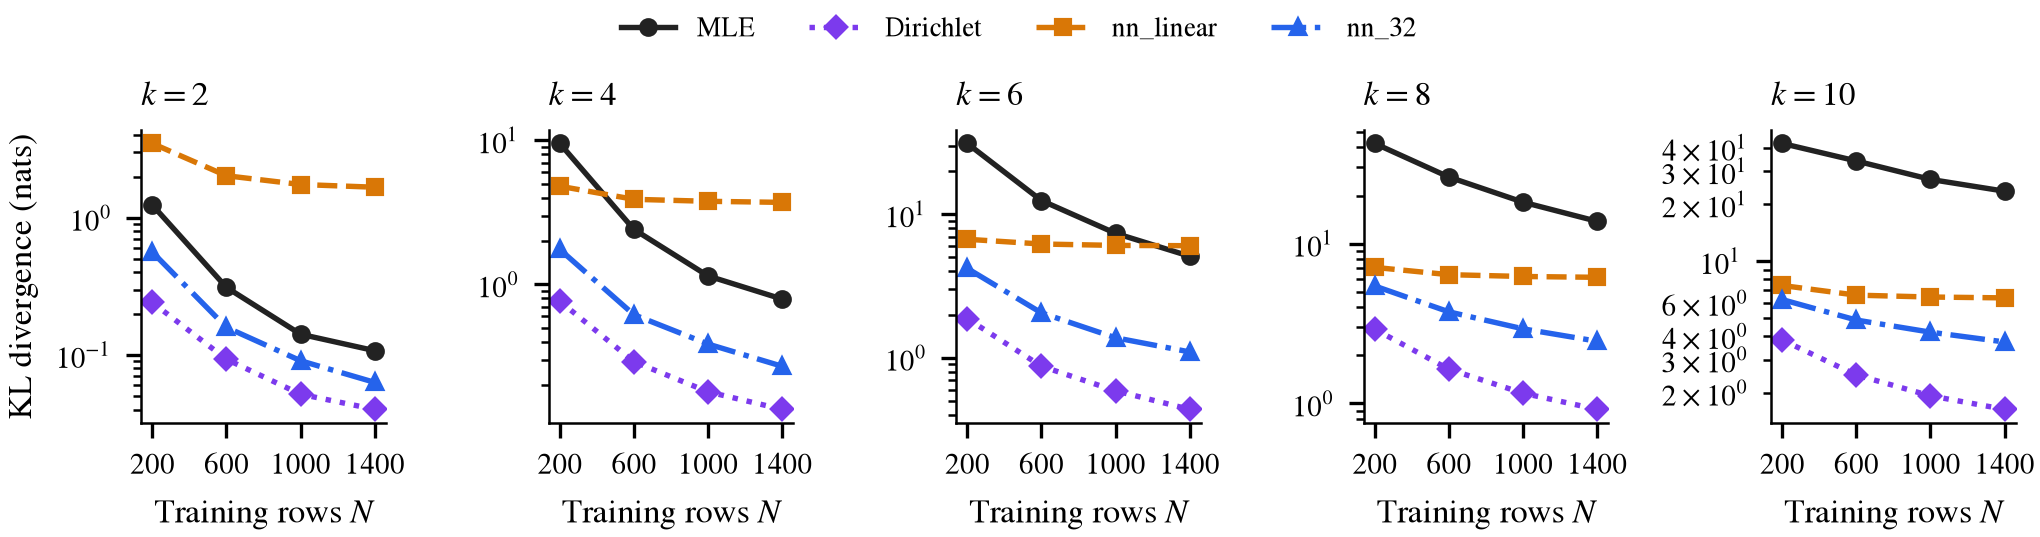
\includegraphics[width=\textwidth]{figs/kl_vs_N_c2.png}
\caption{KL divergence against training rows at each in-degree ($r=2$, 30-node networks, mean over five DAGs; log-scaled y-axis). Standard errors across the DAGs are 1--14\% of each mean, smaller than the markers.}\label{fig:klN}
\end{figure*}

In-degree, cardinality and sample size all act on the estimators through the number of rows per parent configuration, $\rho=N/r^k$ (Eq.~\ref{eq:rho}). Figure~\ref{fig:rho} plots the ratio of each tabular estimator's KL divergence to that of \texttt{nn\_32} against $\rho$, with one line per in-degree. If $\rho$ captured all three factors, every line would fall on a single curve. Against MLE (panel a), whose ratios depend on the floor applied to its zero probabilities (Section~\ref{sec:eval}), the $r=2$ settings come close to this: the ratio falls from about 6--7 at $\rho\leq1$ to about 2.3 at $\rho=250$--$350$.

Cardinality is not fully absorbed, since at the same $\rho$ the ratio is higher at $r=4$ (10.9 against 7.2 at $\rho=0.78$). Below $\rho\approx1$ the $r=4$ ratio falls again, because when almost no configuration is observed both estimators stay close to their uninformed defaults. The advantage over MLE is therefore largest at roughly one training row per parent configuration. With much less data neither estimator can learn much, and with much more, MLE's tables are well estimated.

\begin{figure*}[pos=tbp]
\centering
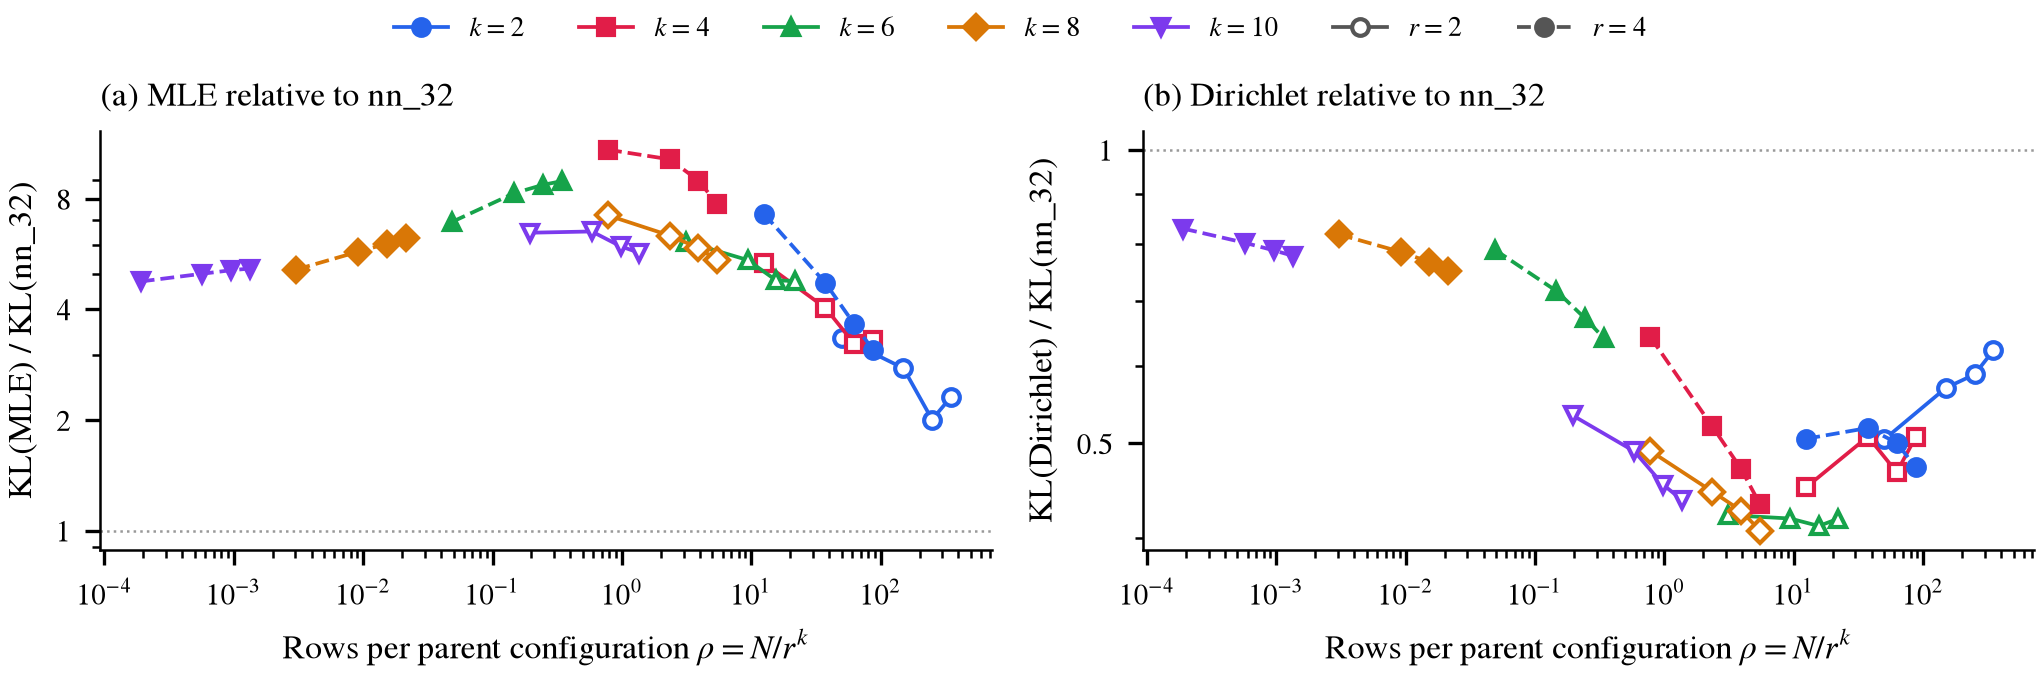
\includegraphics[width=\textwidth]{figs/rho.png}
\caption{Ratio of (a) MLE's and (b) the Dirichlet estimator's KL divergence to that of \texttt{nn\_32}, against rows per parent configuration $\rho = N/r^k$. Each line joins the four sample sizes ($N\in\{200,600,1000,1400\}$) at one in-degree; open markers and solid lines are $r=2$, filled markers and dashed lines $r=4$. Each point is the mean per-DAG ratio over 15 DAGs (five each at 10, 20 and 30 nodes, $\alpha=0.5$; log-scaled axes). Values above 1 favour \texttt{nn\_32}. Panel (a) uses MLE's divergence with zero probabilities floored at $10^{-12}$; a larger floor would lower its ratios.}\label{fig:rho}
\end{figure*}

Against the Dirichlet estimator (panel b), the ratio is below 1 at every setting, from 0.41 to 0.62 at $r=2$ and from 0.43 to 0.83 at $r=4$. This is expected, because the matched-prior reference minimises expected KL divergence on these ground truths, so the ratio measures how far \texttt{nn\_32} remains from the best achievable estimate. The advantage does not come from knowing $\alpha$: the Laplace estimator, which does not use it, has on average 7\% higher KL divergence than the reference and still beats \texttt{nn\_32} in all 500 $r=2$ configurations.

\subsubsection{Ground Truths with Shared Structure}

Figure~\ref{fig:structured} repeats the comparison on the logistic ground truths, where data observed under one parent configuration is informative about others. The ordering now depends on in-degree. At $k=2$ the tables are small and well covered, and the smoothed CPTs remain the most accurate. From $k=6$ upwards, \texttt{nn\_32} is more accurate than every tabular estimator, including the Dirichlet estimator with its pseudocount tuned on validation data, in every configuration at both interaction levels. At $k=10$ the best tabular estimator's KL divergence is 4.4 times that of \texttt{nn\_32} for additive CPDs and 2.4 times with interactions. A table estimates each configuration from its own rows, so it degrades once configurations are rarely observed, whereas a neural CPD can pool the rows of configurations that share a parent's effect.

\begin{figure*}[pos=tbp]
\centering
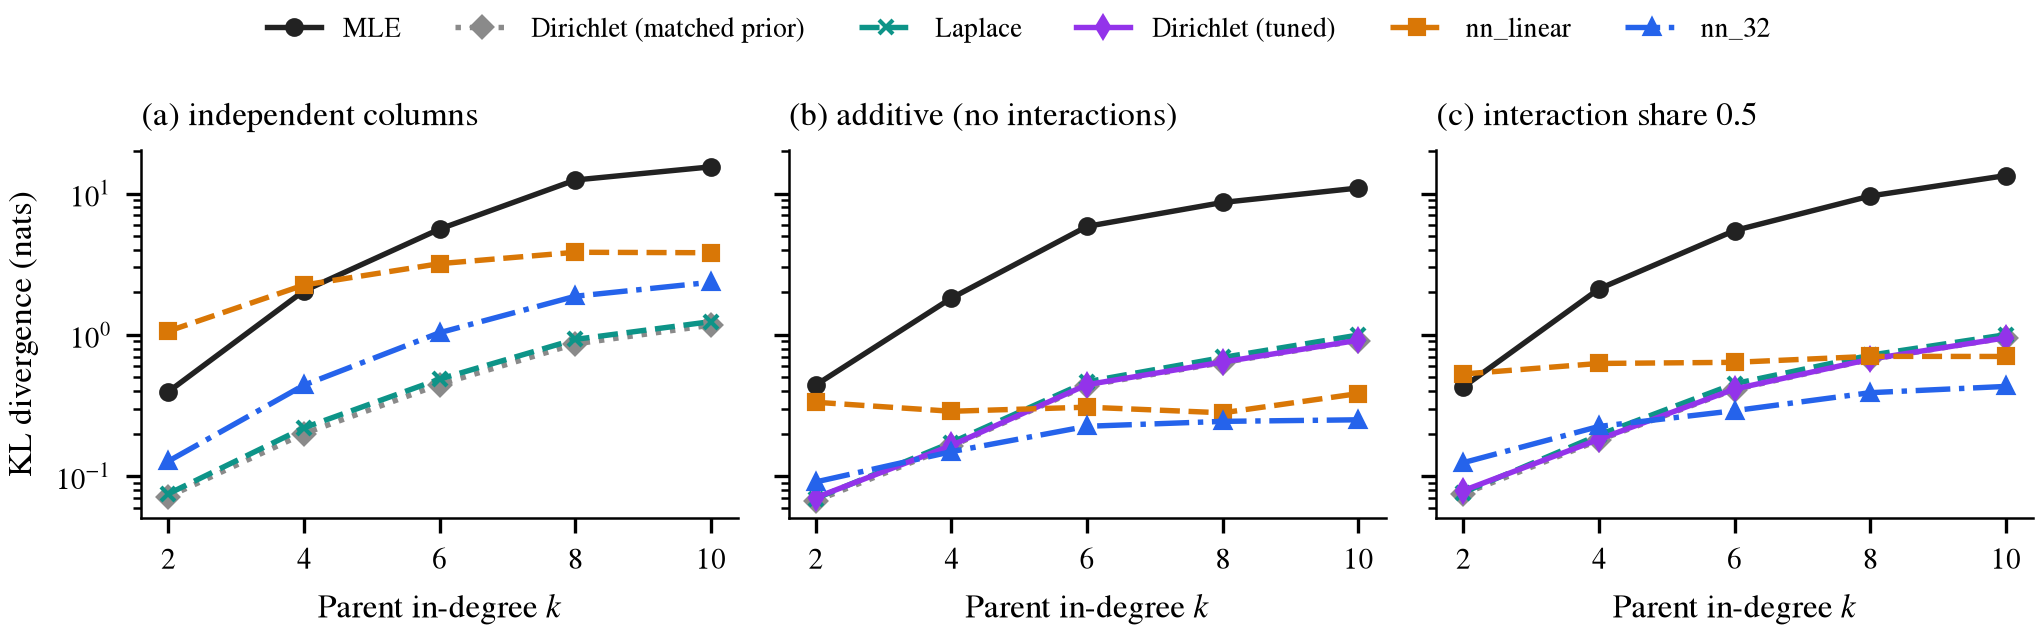
\includegraphics[width=\textwidth]{figs/structured.png}
\caption{Logistic ground truths whose CPTs share structure across parent configurations ($r=2$, 20-node networks, mean over $N\in\{200,600,1000,1400\}$ and five DAGs; log-scaled y-axis): (a) purely additive CPDs, (b) half of the score variance from pairwise parent interactions. The tuned Dirichlet estimator has its pseudocount chosen on validation data.}\label{fig:structured}
\end{figure*}

The interaction level separates the two neural CPDs. With interactions, \texttt{nn\_32} beats the linear softmax in every configuration, because an additive model cannot represent the pairwise terms. For additive CPDs the linear softmax has the right functional form, and it beats every tabular estimator at $k\geq8$, although, being untuned and limited to 200 epochs, it is often still improving when training stops. Together with the independent-column results, this indicates that the advantage of neural CPDs comes from structure shared across parent configurations: where that structure is absent, matched smoothing is optimal, and where it is present, neural CPDs win once the tables become sparse.

\subsection{Real Clinical Data}

On the clinical data the true distributions are unknown, so the estimators are compared on held-out log-likelihood and on how well they diagnose diabetes.

\subsubsection{Predictive Performance}\label{sec:realperf}

Figure~\ref{fig:realmean} shows held-out log-likelihood averaged over all nine combinations of discretisation and DAG. Plain MLE is far below every other estimator at small $N$, because unseen child states receive near-zero probability. Both tuned networks outperform the tuned Dirichlet estimator in all 108 combinations of discretisation, DAG, $N$ and fold (smallest margin 0.004 nats per row), and the untuned linear softmax does so in 105. The three networks perform almost identically: on average \texttt{nn\_32} is 0.004 nats per row better than the linear softmax and 0.019 better than \texttt{nn\_128\_64}.

\begin{figure}[pos=tbp]
\centering
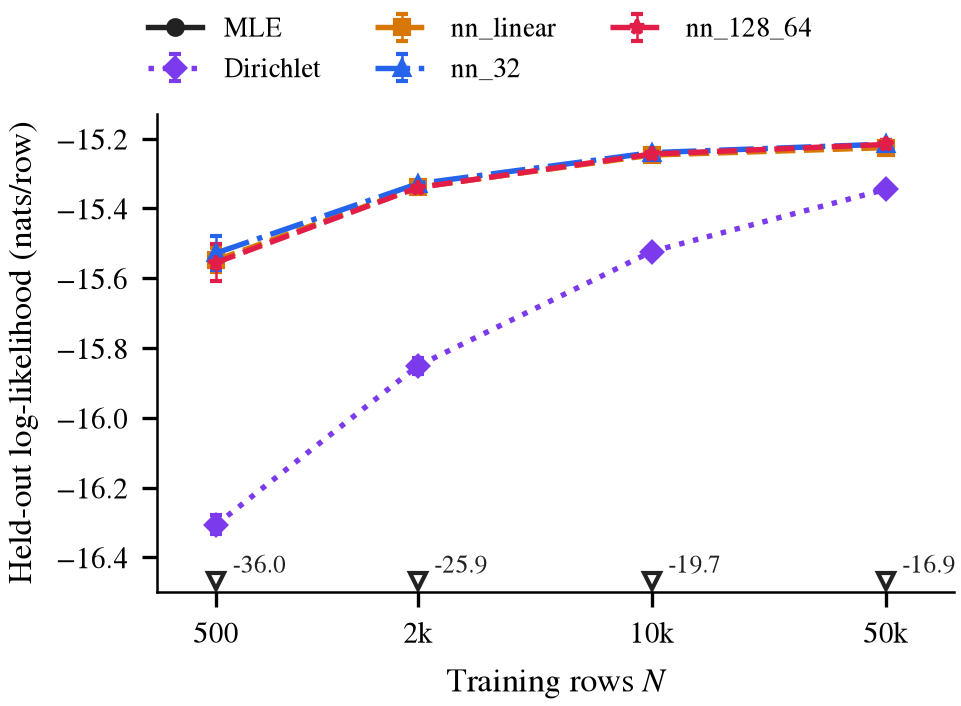
\includegraphics[width=\columnwidth]{figs/real_mean.png}
\caption{Held-out log-likelihood per row, mean over all nine settings and three folds, for each fold's tuned configurations; the linear softmax is untuned (higher is better; log-scaled x-axis).}\label{fig:realmean}
\end{figure}

\begin{table}[tbp]
\caption{Gain in held-out log-likelihood of \texttt{nn\_32} over the tuned Dirichlet estimator (nats per row; mean $\pm$ s.e.\ of the paired differences over three DAG confidence levels and three folds). Every one of the 108 underlying differences is positive.}\label{tab:realgain}
\begin{tabular*}{\tblwidth}{@{\extracolsep{\fill}}lrrrr@{}}
\toprule
 & $N=500$ & 2\,000 & 10\,000 & 50\,000 \\
\midrule
L1 & $0.35\pm0.04$ & $0.20\pm0.03$ & $0.08\pm0.02$ & $0.03\pm0.01$ \\
L2 & $0.84\pm0.05$ & $0.56\pm0.05$ & $0.31\pm0.05$ & $0.14\pm0.03$ \\
L3 & $1.03\pm0.06$ & $0.71\pm0.05$ & $0.43\pm0.05$ & $0.21\pm0.04$ \\
\bottomrule
\end{tabular*}
\end{table}

Table~\ref{tab:realgain} gives the gain of \texttt{nn\_32} over the Dirichlet estimator for each discretisation and sample size. It is largest at fine discretisation and small $N$, and falls as data grows, to 0.005 nats per row for L1 with the high-confidence graph at $N=50\,000$. Finer discretisation and denser graphs both widen the gap, which reaches about 1.15 nats per row for L3 with the low-confidence graph at $N=500$ (Supplementary Figure~S6). The pattern follows data coverage. With 50\,000 rows, only 4\% (L1), 16\% (L2) and 28\% (L3) of test rows meet a parent configuration never seen in training (Supplementary Figure~S7), so most CPT entries are estimated from enough rows that sharing adds little.

Unlike in the synthetic experiments, the linear softmax is competitive with the hidden-layer networks on real data. Survey variables such as age, income and body mass index are ordinal and act on outcomes in largely monotone ways that an additive model can capture, whereas the synthetic CPT columns were drawn independently.

\subsubsection{Diagnostic Accuracy}

Held-out log-likelihood weighs all 22 variables equally, whereas a diagnostic model is judged on the query it is used for. Figure~\ref{fig:diag} shows how well each fitted network predicts diabetes from the other 21 variables. Both neural CPDs are better than the tuned Dirichlet estimator on both measures in all 108 combinations. Their AUROC is already about 0.78 with 500 training rows and 0.81 with 50\,000, whereas the Dirichlet estimator reaches 0.64 and 0.74. Its predictions are also poorly calibrated: in 83 of the 108 combinations its log-loss is worse than that of always predicting the 13.9\% prevalence, which never happens for the networks.

\begin{figure}[pos=tbp]
\centering
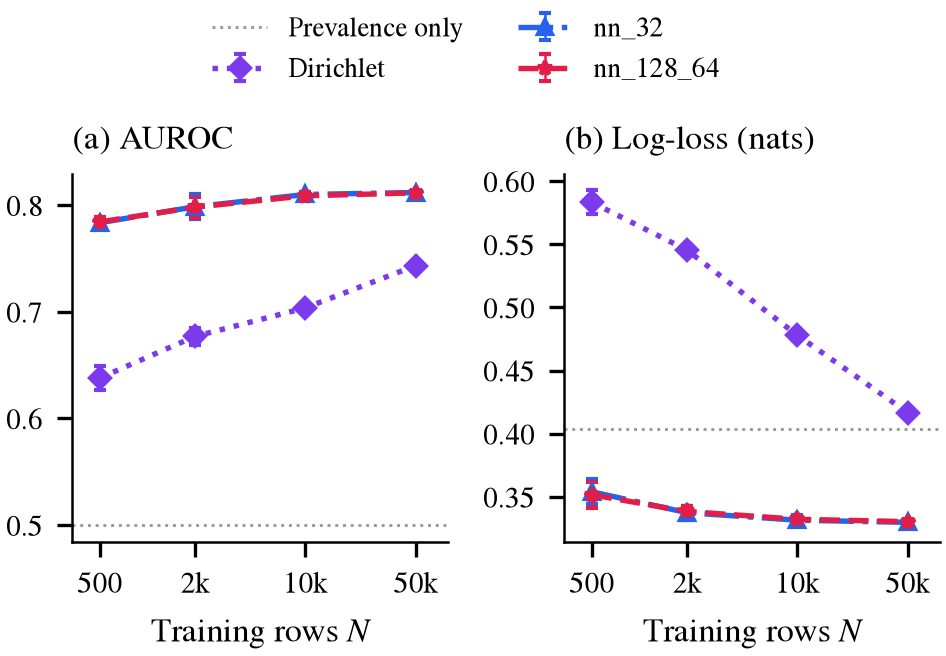
\includegraphics[width=\columnwidth]{figs/real_diagnosis.png}
\caption{Diagnostic accuracy of the predicted probability of diabetes given all other variables, for each fold's tuned configurations: (a) AUROC (higher is better) and (b) log-loss (lower is better), mean over all nine settings $\pm$ s.d.\ over three folds (log-scaled x-axis). The dotted line is the score of always predicting the 13.9\% prevalence. MLE is omitted.}\label{fig:diag}
\end{figure}

The reason is that diagnosis rests on the largest CPT in the network. In every expert DAG the diabetes node has the most parents (7, 8 or 12), and so the most parent configurations, from 864 (L1, high confidence) to almost nine million (L3, low confidence). With 500 training rows, between 42\% (L1) and 92\% (L3) of test patients have a combination of risk factors that never occurs in training. For them a tabular estimator can only give its uninformed default, a 50\% chance of diabetes, far from the true prevalence. A neural CPD instead predicts from the learned effect of each risk factor, so a patient with an unseen combination still receives a sensible probability.

\subsection{Parameter and Training Cost}

Figure~\ref{fig:arms}(b) shows that the networks do not always save parameters. Their size grows only linearly with in-degree, because their input width is the sum of parent cardinalities, but on the synthetic networks the tuned networks still hold more parameters than the tables they replace: \texttt{nn\_256} holds 89\,896 at $k=10$, eight times the CPT's 11\,263. On the real data, whose largest tables are far bigger, the networks are much smaller: at the densest setting, \texttt{nn\_32} holds 13\,364 parameters against the CPT's 9\,016\,841 (Supplementary Figure~S8). What neural CPDs save is data, by sharing statistical strength across parent configurations.

They are not cheaper to fit. In the serial timing run on a 20-node synthetic network, MLE and the smoothed estimators fit in at most 0.3\,s at $r=2$, against 25--119\,s for \texttt{nn\_32}. A network's cost grows with the number of training rows and nodes, and depends on in-degree mainly through early stopping, with training running longest at intermediate in-degree (about 355 epochs at $k=6$, against about 210 at $k=2$ and 245 at $k=10$).

Figure~\ref{fig:timing} shows serial fit time on the real data for three settings spanning the size of the CPTs. The cost of the tabular estimators is set by the size of their tables rather than by $N$: they fit in under a second for the two smaller settings, but MLE and the Dirichlet estimator take about 50\,s and 150\,s for the 9-million-parameter CPT, much of it spent building the tables in pgmpy. The networks instead scale with $N$: \texttt{nn\_32} takes 12--16\,s at $N=500$ and 111--134\,s at $N=50\,000$, and \texttt{nn\_128\_64} up to 285\,s.

\begin{figure*}[pos=tbp]
\centering
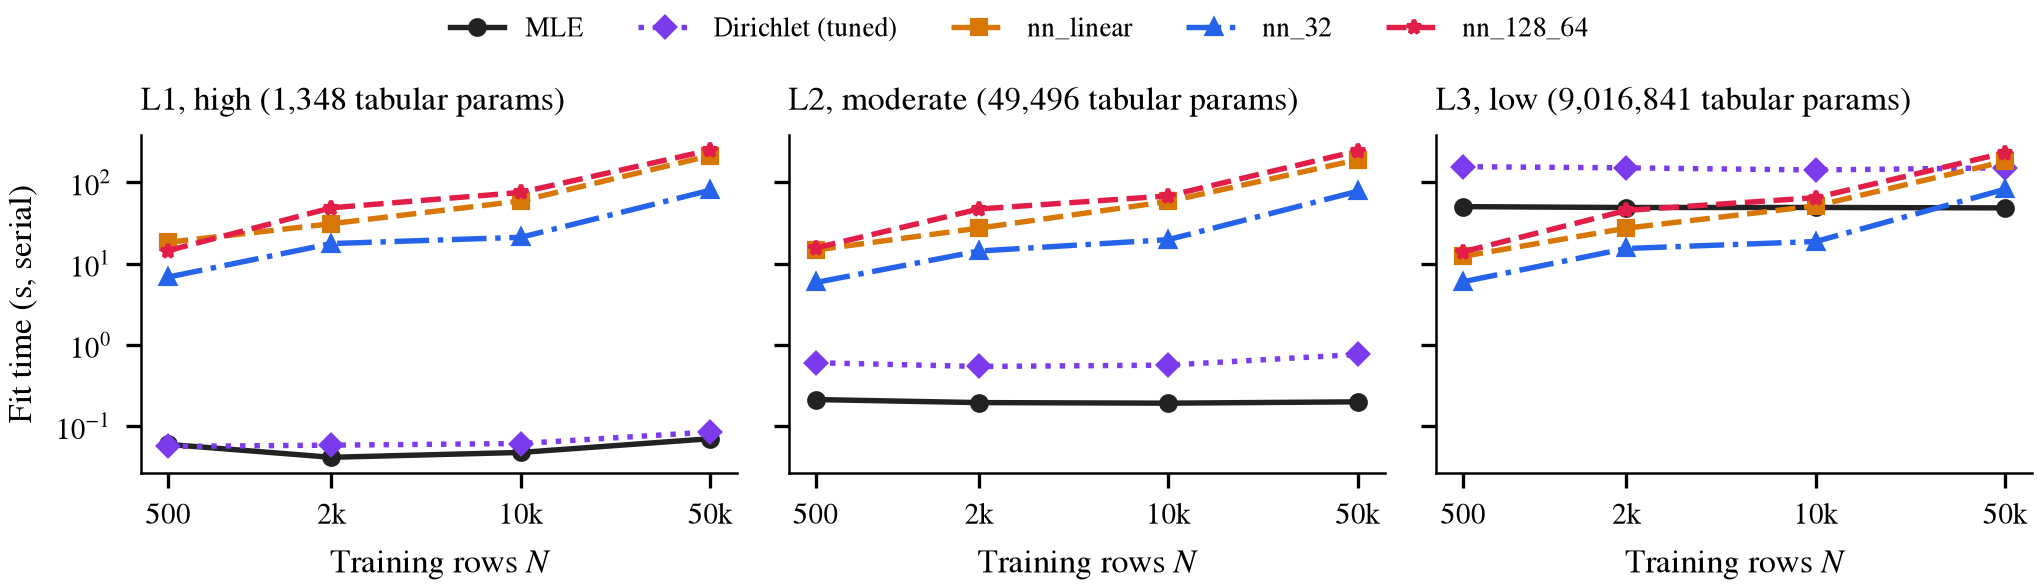
\includegraphics[width=\textwidth]{figs/real_timing.png}
\caption{Fit time on the real dataset from a serial run on one fold, for three discretisation and DAG settings spanning the size of the tabular CPTs (log-scaled axes). The networks are timed with their learning rate before tuning ($6\times10^{-4}$) and the same batch-size rule; the Dirichlet estimator with pseudocount 0.5.}\label{fig:timing}
\end{figure*}

Where the networks are slower, they need far less data for the same accuracy. Table~\ref{tab:realmatch} gives the number of training rows the tuned Dirichlet estimator needs to reach the held-out log-likelihood of \texttt{nn\_32}. Trained on 500 rows, \texttt{nn\_32} is as accurate as the Dirichlet estimator trained on about 1\,400 rows (L1, high confidence) to 34\,000 rows (L3, low confidence), so the table needs between 3 and 67 times as much data. Trained on 2\,000 rows, \texttt{nn\_32} is not matched by the Dirichlet estimator even at 50\,000 rows in three of the nine settings. The two costs are of different kinds: \texttt{nn\_32} spends seconds of computation, while the table needs thousands of additional patient records to match it. Where records are the limiting resource, as in clinical data, this is a favourable exchange.

\begin{table}[tbp]
\caption{Training rows the tuned Dirichlet estimator needs to match the mean held-out log-likelihood of \texttt{nn\_32} trained on $N$ rows (mean over three folds, interpolated on $\log N$ between 500, 2\,000, 10\,000 and 50\,000 rows; rounded to three significant figures). $>$50\,000: not matched within the grid. Each fold on its own gives values within a factor of 1.6 of these.}\label{tab:realmatch}
\begin{tabular*}{\tblwidth}{@{\extracolsep{\fill}}llrrr@{}}
\toprule
 & DAG & $N=500$ & 2\,000 & 10\,000 \\
\midrule
L1 & high & 1\,380 & 6\,650 & 36\,400 \\
 & moderate & 2\,770 & 13\,300 & $>$50\,000 \\
 & low & 5\,210 & 40\,600 & $>$50\,000 \\
L2 & high & 4\,860 & 17\,300 & $>$50\,000 \\
 & moderate & 10\,700 & 48\,000 & $>$50\,000 \\
 & low & 21\,700 & $>$50\,000 & $>$50\,000 \\
L3 & high & 6\,120 & 29\,400 & $>$50\,000 \\
 & moderate & 15\,500 & $>$50\,000 & $>$50\,000 \\
 & low & 33\,700 & $>$50\,000 & $>$50\,000 \\
\bottomrule
\end{tabular*}
\end{table}

\subsection{Summary of Findings}

On synthetic networks whose distributions share no structure across parent configurations, no estimator can gain by sharing, and the matched-prior Dirichlet estimator is optimal. Neural CPDs, which are not told that prior, stay within about two and a half times its divergence and beat unsmoothed MLE in 793 of 800 configurations, with their largest advantage over MLE at about one training row per parent configuration. When the distributions do share structure, neural CPDs beat every tabular estimator from in-degree 6 upwards, including one with its pseudocount tuned on validation data, and a hidden layer is needed once parents interact.

On the clinical data, both networks beat the tuned Dirichlet estimator in all 108 comparisons, most clearly at fine discretisations and small samples. They also diagnose diabetes better, with an AUROC of about 0.81 against 0.74 at 50\,000 rows, because the diabetes node has the largest table in every expert graph. The networks take seconds to minutes to fit, longer than most tables, but a table needs 3 to 67 times as much data to match them.

% ===========================================================================
\section{Conclusion}\label{sec:conclusion}
% ===========================================================================

Bayesian networks are a promising framework for medical diagnosis because their graphical structure makes probabilistic reasoning visible, but their standard estimators learn every parent configuration from its own observations and become unreliable when data is scarce relative to the number of configurations. This report replaced the conditional probability tables with neural CPDs while keeping the graph that makes the network interpretable.

On synthetic networks in which each configuration's distribution is unrelated to the others, a smoothed table matched to the generating process is the best possible estimator. Neural CPDs came close to it without being told how the data were generated, and far outperformed unsmoothed maximum likelihood. When configurations do share structure, as clinical risk factors plausibly do, neural CPDs were more accurate than every table once nodes had many parents, and a hidden layer was needed when parents interact. The clinical data showed the same: neural CPDs were more accurate than a tuned smoothed table in every setting, and diagnosed diabetes far more accurately, because the diabetes node depends on the largest table in every expert graph. Fine clinical categories therefore need not be collapsed to keep tables estimable. The benefit is statistical rather than computational: a neural CPD costs more to train, but needs far less data to estimate the same distribution well.

\subsection{Limitations}

The independent-column synthetic networks contain no structure shared across parent configurations and so favour smoothed tables by construction, and the structured ground truths cover only $r=2$, 20-node networks and two interaction levels. Neither reproduces the noise or class imbalance of clinical data. Network settings were tuned on 20-node networks, and on real data the networks reuse the $r=4$ settings with only the learning rate tuned. The selected learning rate and pseudocount are the largest values in their grids, and the real-data comparison rests on three folds. Finally, a neural CPD is less directly readable than a CPT: the graph remains interpretable, but each local distribution has to be queried rather than read off a table.

\subsection{Future Work}

The most natural extension is to hybrid networks. Many physiological measurements, such as blood pressure and glucose, are continuous, and discretising them loses information. \citet{Gaogle2026} showed that neural CPDs work for Gaussian Bayesian networks, and combining the two approaches would let clinical variables be modelled in their natural form. Richer clinical data, such as critical care databases with many more variables and rarer conditions, would test neural CPDs in the regime of few rows per configuration where they were most valuable here. Monotonicity or sign constraints elicited from clinicians could encode accepted medical relationships in the networks directly. Finally, the diagnostic query here observes every other variable and so needs only the Markov blanket of the diagnosis node; queries with partial evidence require inference through the whole network, for example by generating a neural CPD's table on demand, and evaluating them would test whether the gains carry through to clinical decision support.

\section*{Code and Data Availability}

The code for every experiment, the results files, and the notebooks that produce each figure and table in this report are available at \url{https://github.com/kay-asp/Neural-Discrete-Bayesian-Network}. The CDC Diabetes Health Indicators data are available from the UCI Machine Learning Repository \citep{cdc_diabetes_2023}, and the expert-elicited DAGs from \citet{zahoor2025investigatingvaliditystructurelearning}; copies of both are included in the repository.

\section*{Supplementary Material}

The supplementary material contains the architecture-selection results and the settings of every estimator, the moderate-confidence expert DAG, the synthetic results for each network size, and the real-data results, unseen-configuration rates and parameter counts for each discretisation and DAG.

\section*{Ethics and Data Use}

This project involves no human participants. The real-data experiments use the CDC Diabetes Health Indicators dataset \citep{cdc_diabetes_2023}, an anonymised, publicly available extract of the 2015 Behavioral Risk Factor Surveillance System survey collected by the US Centers for Disease Control and Prevention and redistributed by the UCI Machine Learning Repository from a public-domain release (Creative Commons CC0 1.0). It contains no identifiers. The synthetic data are sampled from randomly generated networks over abstract variables. The project was classified as no risk and received an ethics waiver from the School of Computer Science and Applied Mathematics at the University of the Witwatersrand, under the University's Human Research Ethics Committee (Non-Medical) (waiver number WCSAM-2026-48).

\section*{AI-Use Declaration}

Anthropic's Claude Opus 5.5 was used to assist with writing and debugging code, reviewing related literature, drafting and editing text, checking the code and drafts for consistency, and preparing figures and document layouts. The experimental design and the interpretation of the results are the author's own, and every reported number was produced by the code in the accompanying repository. All AI-assisted code and text was checked by the author, who takes responsibility for the content and conclusions of this report.

\bibliographystyle{cas-model2-names}
\bibliography{references}

\end{document}
